\chapter{Linear Theory}

\section{Introduction}
In this chapter we extend the results of Billant and Chomaz \cite{2000c} to the sub-buoyancy length-scales. We also reproduce the numerical results presented by Billant and Chomaz and confirm their conclusions about the existence of the zigzag instability at the buoyancy scale. 

\section{Results}
The equations that we want to solve are the linear Boussinesq equations, which we derived in Chapter 2 and we use the numerical scheme discussed in Chapter 3. We repeat the equations here for reference. 

(insert equations)

In our simulations, we investigate a range of Reynolds numbers $Re=5000-20{,}000$ and Froude numbes $F_{h}=0.05-0.02$. These numbers have been chosen since they are within the range of the results of Billant and Chomaz, who investigate a similar range. We additionally consider a Schmidt number to be unity which is a standard practice (cite... justify? numerically difficult?). 

For our simulations a box size of $L=9$ with $N=512$ grid points used. The reason for choosing $L=9$ was such that there was no possibility of the fields interacting with itself across the periodic boundary. As discussed previous, a box size as small as $L=5$ could be used and $L=4$ has been used in practice (cite), however we erred on the side of caution and repeated the box size conditions of Billant and Chomaz \cite{bc2000c}.  The timesteps of $\Delta t=0.000950$ for $F_{h}=0.2,Re=2000,5000,10000$ and $\Delta t=0.000375$ for all the other simulations. These were chosen following Billant and Chomaz \cite{bc2000c}. 

Unlike Billant and Chomaz\cite{bc2000c} we did not restart each simulation with the previous eigenmode because we used a parallel approach for evaluating multiple $k_{z}$ simultaneously. We investigate a range of Froude and Reynolds number and a wide range of $k_{z}$ from $1$ to $200$ depending on the Froude and Reynolds number. This wavenumber range incorporates the scale of the zigzag instability down to the viscous damping scale. 

The code was written in Fortran and all the FFTs were done by FFTW (Cite) and was tested by comparing sigma 

\section{Growth Rate Results}
Fig.~\ref{FixFhVaryRe} shows the largest eigenmode growth rate as a function of vertical wavenumber for fixed $F_{h}$ and $Re$. Following Billant and Chomaz\cite{bc2000c}, the scaled vertical wavenumber $k_{z}F_{h}$ is employed. The qualitative behaviour for the growth rates at different Reynolds numbers are very similar to one another. At small $k_{z}$, the growth rate reaches a local maximum, the zigzag peak, located at $k_{z}F_{h}\approx 0.6$ as predicted by Billant and Chomaz\cite{bc2000c}.  The growth rate then decreases for increasing $k_{z}$ to a local minimum before increasing to a second local maximum. Continuing to even smaller vertical scales, viscous effects increase and may damp out the instability, and hence the growth rate decays with increasing $k_{z}F_{h}$ in the limit of large $k_{z}F_{h}$. Oscillatory growth rates are observed for the smallest $k_{z}F_{h}$ as observed in Ref 26\nocite{bc1999}. The imaginary part of the growth rate $\sigma_{i}$ remains zero everywhere else except in a small region surrounding the local minimum between the zigzag and short-wave peaks. This oscillatory behaviour is not considered here. 

For $F_{h}=0.2$ (Fig.~\ref{FixFhVaryRe}a), the peak growth rate of the short-wave instability exceeds that of the zigzag instability for increasing Reynolds numbers. The growth rates at the second peak is smaller for $F_{h}=0.1$ (Fig.~\ref{FixFhVaryRe}b), but they continue to increase with increasing $Re$. For $F_{h}=0.05$ (Fig.~\ref{FixFhVaryRe}c), the second peak is weaker than the zigzag peak. Fig.~\ref{FixReVaryFh} shows the growth rate for fixed Reynolds numbers with varying Froude numbers. Examining the case of $Re=20000$ (Fig.~\ref{FixReVaryFh}a), the second peak increases with increasing Froude. A similar result is observed for $Re=10000$ and $5000$ (Fig.~\ref{FixReVaryFh}b-c). $Re=2000$ is not included because viscous effects have damped out the second peak in this case. Overall, the dependence of the short-wave growth rate on Froude is also more pronounced then that of Reynolds. For example, the growth rate of the second peak at fixed $Re=20000$ (Fig.~\ref{FixReVaryFh}a) doubles from $F_{h}=0.05$ to $F_{h}=0.2$. By contrast, at fixed $F_{h}=0.2$ (Fig.~\ref{FixFhVaryRe}a), the increase in the growth rate from $Re=5000$ to $Re=20000$ is only about $25\%$ larger. 

%\begin{figure}
%\begin{center}
%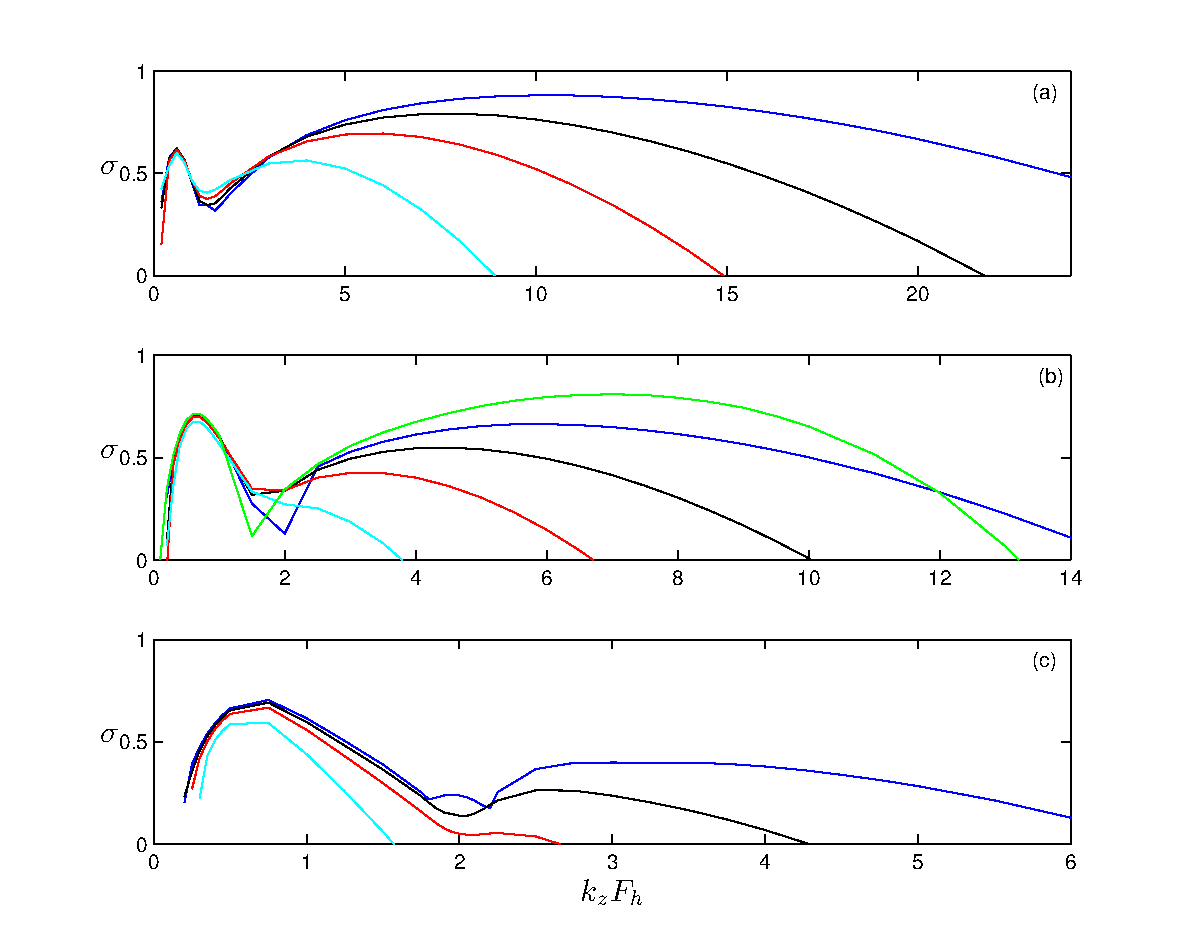
\includegraphics[width=\textwidth]{fixed_froude_varying_reynolds.eps}
%\caption{Growth rate $\sigma$ as a function of $k_{z}F_{h}$ for fixed $F_{h}=$(a) $0.2$, (b) $0.1$, (c) $0.05$ with Re$=2000$ (cyan), Re$=5000$ (red), Re$=10000$ (black), Re$=20000$ (blue). In panel (b) the green line is the hyperviscosity case with $Re=20000$.}
%\label{FixFhVaryRe}
%\end{center}
%\end{figure}
%\begin{figure}
%\begin{center}
%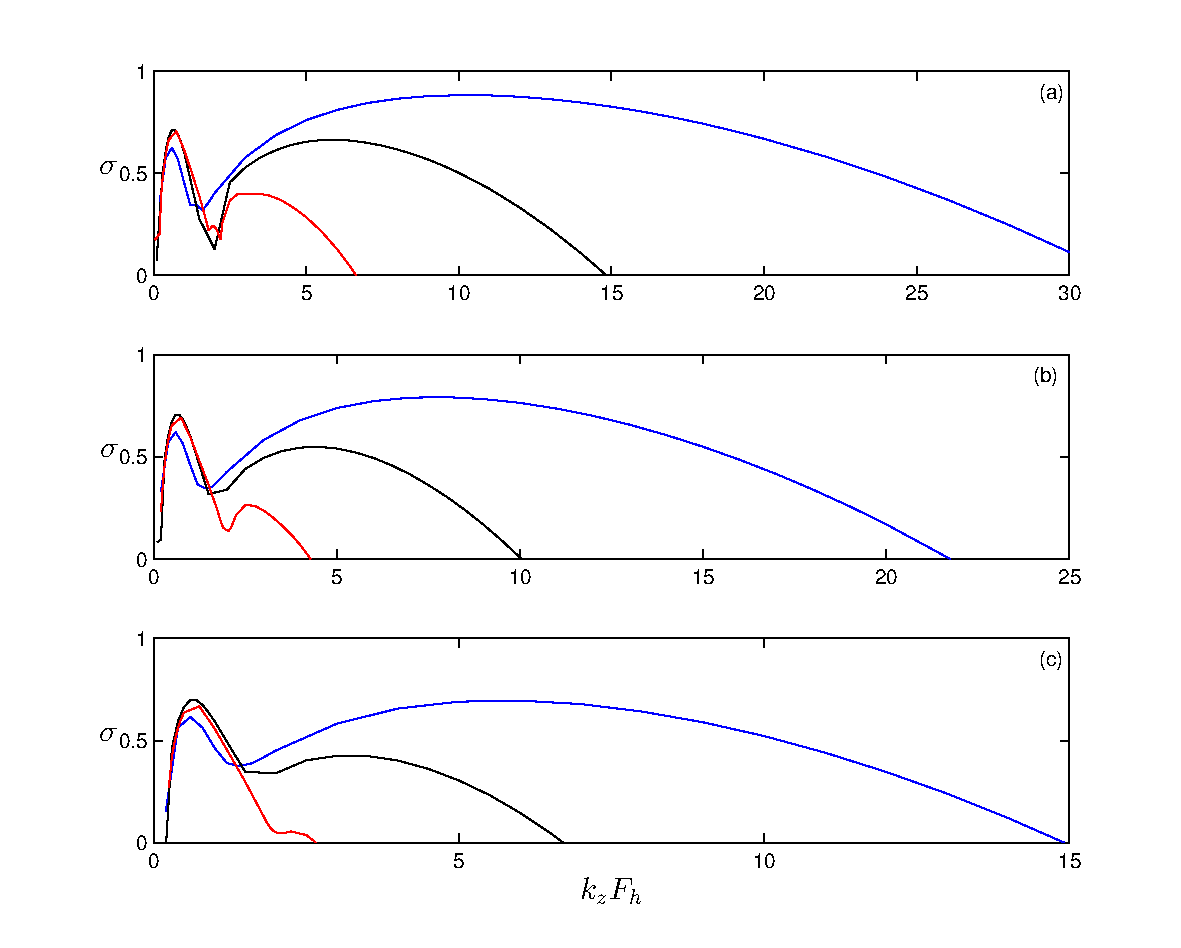
\includegraphics[width=\textwidth]{fixed_reynolds_varying_froude.eps}
%\caption{Growth rate $\sigma$ as a function of $k_{z}F_{h}$ for fixed $\text{Re}=(a) 20000, (b) 10000, (c) 5000$ with $F_{h}=0.05$ (red), $F_{h}=0.1$ (black), $F_{h}=0.2$ (blue).}
%\label{FixReVaryFh}
%\end{center}
%\end{figure}
The above analysis demonstrates that the short-wave growth-rate peak moves to larger $k_{z}F_{h}$ with increasing $F_{h}$ and increasing $Re$, but has a stronger dependence on Froude than Reynolds. Some of this joint dependence can be explained by examining the dependence on the buoyancy Reynolds number $Re_{b}=F_{h}^{2}Re$ \cite{riley2003,hebert2006,brethouwer2007}. In stratified turbulence, the buoyancy Reynolds number is analogous to the Reynolds number in the viscous term due to the vertical gradients \cite{brethouwer2007}. As $k_{z}$ increases, we move to smaller vertical scales where the vertical viscosity terms, controlled by the buoyancy Reynolds number, dominates, so it follows that the second peak may be governed by $Re_{b}$. In Fig.~\ref{Buoy} the location of the second peak from Fig.~\ref{FixFhVaryRe} is plotted as a function of the buoyancy Reynolds number. The peak location line is approximately linear and can be fitted with the curve $k_{z}F_{h}= Re_{b}^{2/5}$, which is plotted. This scaling implies that the vertical wavenumber, $k_{z}$, of the short-wave instability is approximately 
\begin{align}
k_{z} \sim F_{h}^{-1/5} Re^{2/5}\label{buoyscale}.
\end{align} 
The dependence of the growth rate on $k_{z}F_{h}$ appears to be similar in the cases with different $F_{h}$ and $Re$ but the same $Re_{b}$. Fig.~\ref{ReBuoy} demonstrates the similarity of the growth rate plotted against $k_{z}F_{h}$ for two cases with $Re_{b}=500$ and two cases with $Re_{b}=50$. For both cases, the locations of the zigzag and second peak line up quite well. The difference between the red and blue curves at the second peak is $4\%$ for $Re_{b}=200$ and $6\%$ for $Re_{b}=50$, a reasonable variation. 

% It is interesting to note that the red curve, corresponding to $Re=20000$ and $F_{h}=0.1$ (a), $F_{h}=0.05$ (b), is lower then the blue curve, corresponding to $Re=5000$ and $F_{h}=0.2$ (a), $F_{h}=0.1$ (b). This supports the observation, and is clear from the definition of the buoyancy Reynolds number, that the stratification may play a more important role in the instability than the viscosity.   

%\begin{figure}
%\begin{center}
%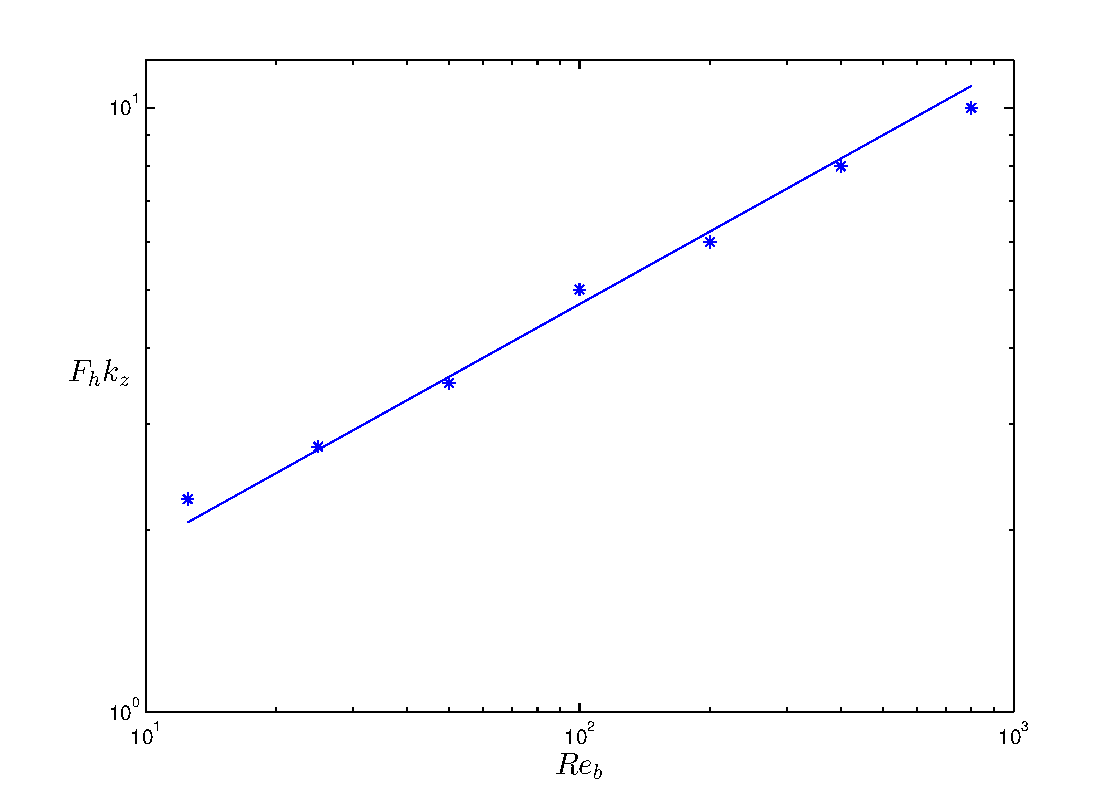
\includegraphics[scale=0.6]{second_peak_buoyancy.eps}
%\caption{The location of the second peak as a function of the buoyancy Reynolds number $Re_{b}$. $k_{z}F_{h}$ is taken from Fig.~\ref{FixFhVaryRe}. The straight line is $Re_{b}^{2/5}$.}
%\label{Buoy}
%\end{center}
%\end{figure}
%\begin{figure}
%\begin{center}
%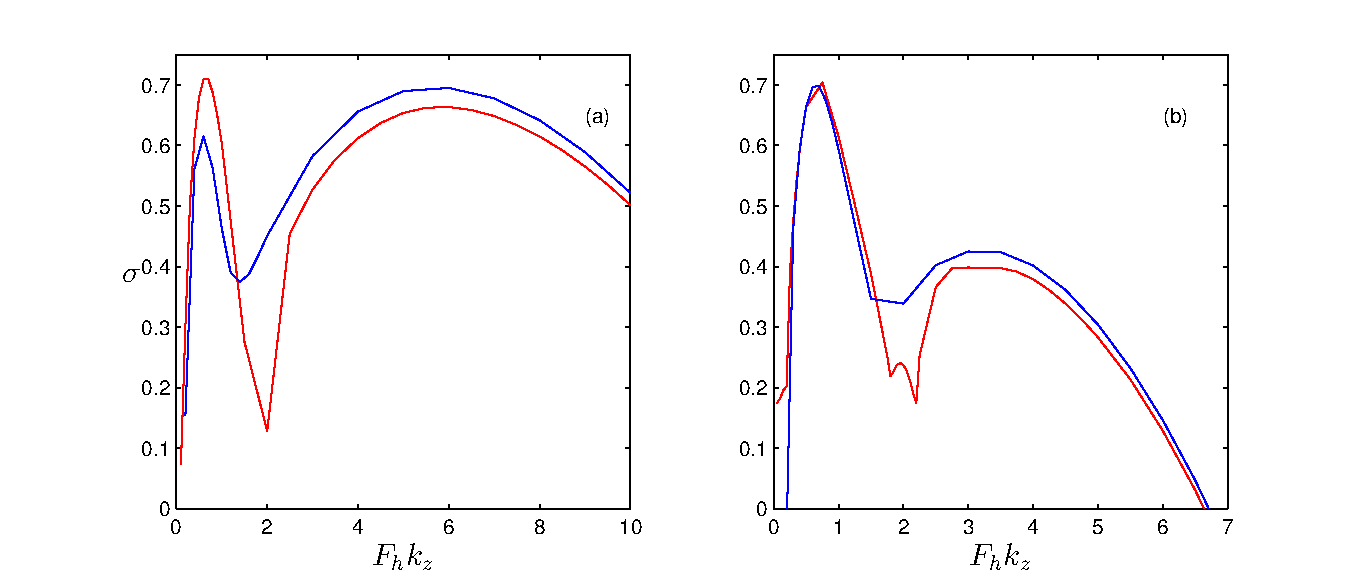
\includegraphics[width=\textwidth]{buoyancy_reynolds.eps}
%\caption{Growth rate $\sigma$ as a function of $F_{h}k_{z}$ for fixed $Re_{b}$. In (a), red is $Re=20000, F_{h}=0.1$ and blue is $Re=5000, F_{h}=0.2$, both corresponding to $Re_{b}=500$; in (b) red is $Re=20000, F_{h}=0.05$ and blue is $Re=5000, F_{h}=0.1$, both correpsonding to $Re_{b}=50$.}
%%\caption{Growth rate $\sigma$ as a function of $k_{z}$ for fixed $Re_{b}=(a) 200, (b) 50$. In (a) red corresponds to $Re=20000, F_{h}=0.1$ blue to $Re=5000, F_{h}=0.2$, in (b) red corresponds to $Re=20000, F_{h}=0.05$, blue $Re=5000, F_{h}=0.1$}
%\label{ReBuoy}
%\end{center}
%\end{figure}


In Fig.~\ref{FixFhVaryRe} (b) the green curve corresponds to a hyperviscosity run with $Re=20000$, which has $Re_{h}=2.8\times 10^{8}$. The motivation for using hyperviscosity is to capture higher-Reynolds number regime by restricting dissipation to only the largest wavenumbers. As the hyperviscosity run demonstrates, the zigzag peak is independent of Reynolds number and the existence of the peak would be expected at higher Reynolds numbers. For the second peak, we note that the growth rate  of the hyperviscosity run exceeds that of $Re=20000$ for $k_{z}F_{h}>3$ and reaches a maximum around $k_{z}F_{h}=7$. The maximum growth rate in the hyperviscosity case is around $25\%$ larger than the regular viscosity case with $Re=20000$. At $k_{z}F_{h}=12$ we see the hyperviscosity and non-hyperviscosity curves cross. This intersection corresponds to the horizontal wavenumber at which the hyperviscosity damping rate equals the regular viscous damping rate for $Re=20000$. For $k_{z}$ greater than this maximum, the hyperviscosity operator experiences greater damping than the regular viscosity, which can be seen by the sudden drop off of the growth rate. This simulation presents evidence that as $Re\rightarrow \infty$, the growth rate of the second peak will the same order as, or larger than, the growth rate of the zigzag instability. 

\subsection{Structure} 
%\begin{figure}
%\begin{center}
%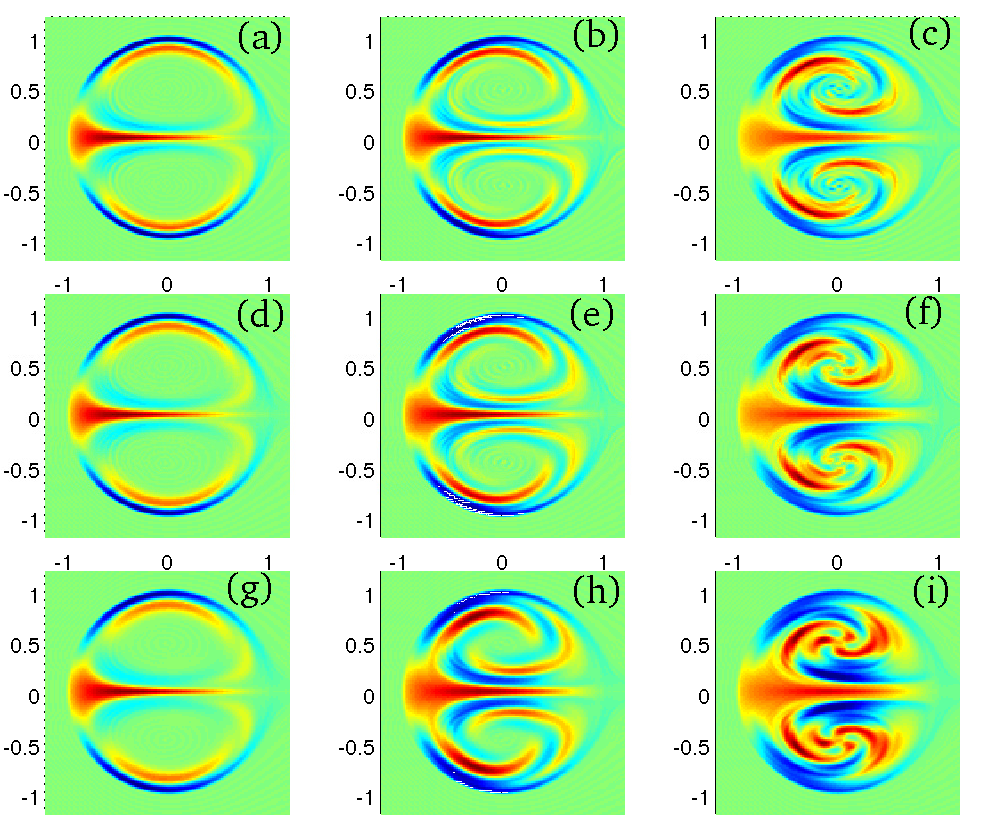
\includegraphics[width=\textwidth]{vorticity_second_peak.eps}
%%\caption{Perturbation vertical vorticity $\omega_{z}$ for $k_{z}$ at the second peak. $F_{h}=(a)(d)(g) 0.2 ,(b)(e)(h) 0.1, (c)(f)(i), 0.05, Re=(a)(b)(c) 20000, (d)(e)(f) 10000, (g)(h)(i) 5000$.}
%\caption{Perturbation vertical vorticity $\omega_{z}$ at second peak for $Re=20000\text{ (top) }, 10000 \text{ (middle) }, 5000 \text{ (bottom) }$; and $F_{h}=0.2 \text{ (left) }, 0.1 \text{ (middle) }, 0.05 \text{ (right) }$.}
%\label{secondpeak}
%\end{center}
%\end{figure}
Fig.~\ref{secondpeak} shows the spatial structure of the perturbation vertical vorticity at the second peak for different $Re$ and $F_{h}$. Qualitatively, we observe greater variation for different Froude numbers versus different Reynolds number as suggested above.  At the largest Froude number, the perturbation vorticity is organised in thin strips around and inside the dipole core between the two vortices. Panels (b),(e),(h) have $F_{h}=0.1$ and have a similar overall structure to the larger Froude number. Here, in the cores of the vortices, there is an emergence of a swirl-like pattern. At lower Reynolds number, the structure is spread out due to diffusion, while at higher Reynolds number, small-scale structure is beginning to emerge. This trend continues overall as we move to lower Froude numbers. 

Examining panels (g)-(i) (fixed $Re$ and decreasing $F_{h}$), the core of the dipoles has a twisting-like behaviour as the Froude number decreases. From this we can conclude that the instability structure of the second peak depends more on the Froude number than on the Reynolds number, which again reinforces the buoyancy Reynolds number scaling.  Indeed, if we consider the cases with $Re_{b}=50$ and $200$ as above, which correspond to Fig.~\ref{secondpeak} (b),(g) and (c),(h) respectively, we can see similar structure in the vorticity fields. Additionally, the anti-symmetric structure of the perturbation can be observed in the dominant eigenmodes in all cases, as found by Refs 17,26\nocite{bc1999,bc2000c}.

% The vorticity being very thin in the centre is consistent with the results of \cite{pierrehumbert1986} which examined unstratified inviscid vortices at small vertical scales which also demonstrated this behaviour. 
%\begin{figure}
%\begin{center}
%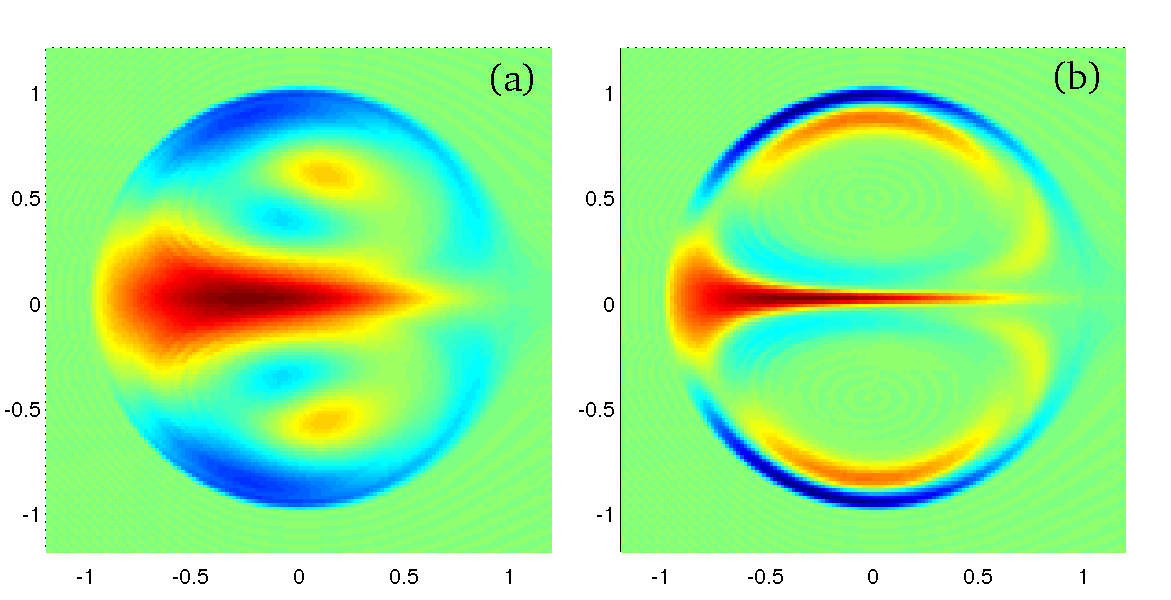
\includegraphics[scale=0.5]{second_peak_vs_zigzag.eps}
%\caption{Perturbed vertical vorticity $\omega_{z}$ at (a) the zigzag peak (b) the second peak for $Re=5000, F_{h}=0.2$}
%\label{zigzagcomparison}
%\end{center}
%\end{figure}

Fig.~\ref{zigzagcomparison} shows the perturbation structure for the zigzag peak (a) and the short-wave peak (b) for the case of $Re=5000,F_{h}=0.2$. This case was chosen because the growth rates of the two wavenumbers is roughly the same (see Fig~\ref{FixFhVaryRe} a). The zigzag instability exhibits a quadropole vorticity structure as discussed in Ref 17\nocite{bc2000c}, which corresponds to a bend and a twist of the basic state dipole. The short-wave instability shares some common overall structure with the zigzag instability. Both have a line of vorticity centred in between two Lamb-Chaplygin vortices and have a ring of vorticity negative vorticity around the outer edges of the dipoles. Additionally, the number of local maximum and minimum remains the same. However, in the short-wave instability, these bands of vorticity have been squeezed into thinner strips and are much more localised along the outer edges of the vortices. In the cores of the dipoles, there is almost no structure and we do not see a quadropole moment. The full vorticity field of the short-wave instability has a much more dominant twist then the zigzag instability and the bending of the dipole is reduced. As the stratification is increased, this behaviour continues but there is a significant emergence of structure within the cores of the vortices, as observed in Fig~\ref{secondpeak}.


\subsection{Subdominant modes?} 
The above analysis only provides the leading eigenvalue. Discuss subdominant mode ideas. Krylov method + matlab method.
\section{Dimensional Analysis}
That will go here. 


\section{Stuff to add}
Stuff about the scaling arugments from the fluid background chapter here.
\section{Conclusion}

